\documentclass[a4paper,utf8]{article}
\usepackage[heading,fancyhdr]{ctex}
\usepackage{amsmath,amssymb,geometry,lastpage,ulem}
\usepackage{array,tabularx,graphicx}
\geometry{
    top=25.4mm, 
    left=30mm, 
    right=30mm, 
    bottom=35mm,
    headsep=5.9mm,
}
\ctexset{
    section = {format+=\raggedright}
}
\newcommand{\expinfo}[5]{
    {\zihao{-3}\bfseries\songti
    实验名称:\uline{\hfill\mbox{#1}\hfill} \\[2.9mm]
    学\quad 号:\uline{\makebox[25mm]{#2}}\hfill
    姓\quad 名:\uline{\makebox[25mm]{#3}}\hfill
    班\quad 级:\uline{\makebox[25mm]{#4}} \\[2.9mm]
    合作者:\uline{\makebox[25mm]{无}}\enspace~
    桌\quad号:\uline{\makebox[25mm]{}}\hfill\mbox{}\\[2.9mm]
    指导教师:\uline{\makebox[30mm]{#5}}\hfill\mbox{} \\[2.9mm]
    实验日期:\uline{\makebox[30mm]{}}\hfill\mbox{} \\[58.7mm]
    }
}%\expinfo{实验名称}{学号}{姓名}{班级}{指导教师}
\pagestyle{fancy}
\fancyhf{} \fancyhead[C]{材料科学基础实验} \fancyfoot[C]{\thepage~/~\pageref{LastPage}}
\begin{document}
\begin{center}
    {\mbox{}\\[7em]\zihao{2}\bfseries\songti%
    材料科学基础实验报告}\\[34mm]
    \expinfo{实验四 碳钢淬火、回火后的组织观察与硬度分析}{22301070}{杨雨燃}{22材物}{杨玉华}
\end{center}
\newpage
\section*{【实验目的】}
    \begin{enumerate}
        \item 了解碳钢的淬火、回火过程。
        \item 观察和研究碳钢经不同淬火、回火处理后显微组织的特点,分析冷却条件、淬火温度及回火条件对其组织形态与硬度的影响,并了解淬火、回火的应用领域。
    \end{enumerate}   
\section*{【实验原理】}%简单描述,含必要的公式和附图;

\textbf{(一) 淬火}

淬火是将钢奥氏体化后以大于临界冷却速度的速度进行冷却,获得马氏体或下贝氏体组织的热处理工艺。其主要目的是为了获得马氏体,提高试样的硬度和强度。

1、淬火温度的选择:
\begin{center}
    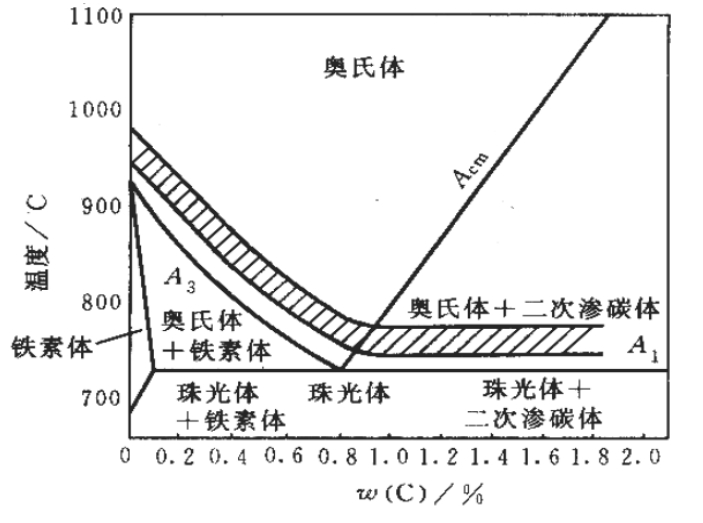
\includegraphics[width=200pt]{1.png}
\end{center}

2、保温时间:保温的目的是使钢件热透,使奥氏体充分转变为均匀化。计算公式为:
\begin{center}
    τ = $\alpha$KD
\end{center}
 
式中,$\alpha$为加热系数;K为装炉系数;D为有效尺寸,mm。

3、淬火冷却介质:钢在加热获得奥氏体后要选用适当的冷却介质进行冷却,获得马氏体组织。常用的冷却介质有油、水、盐水、碱水等,其冷却能力依次增加,但是这些冷却介质都存在不同的缺点。

4、淬火后的组织:

低碳钢淬火后能观察到一束束接近相互平行的细条状马氏体群;

中碳钢淬火将得到细针
状马氏体和板条状马氏体的混合组织;

高碳钢,如共析钢和过共析钢在等温淬火后可得到贝氏体组织;亚共析钢淬火后能观察到板条状或针的状马氏体组织,共析钢和过共析钢在
淬火后亦得到马氏体组织。

\begin{center}
    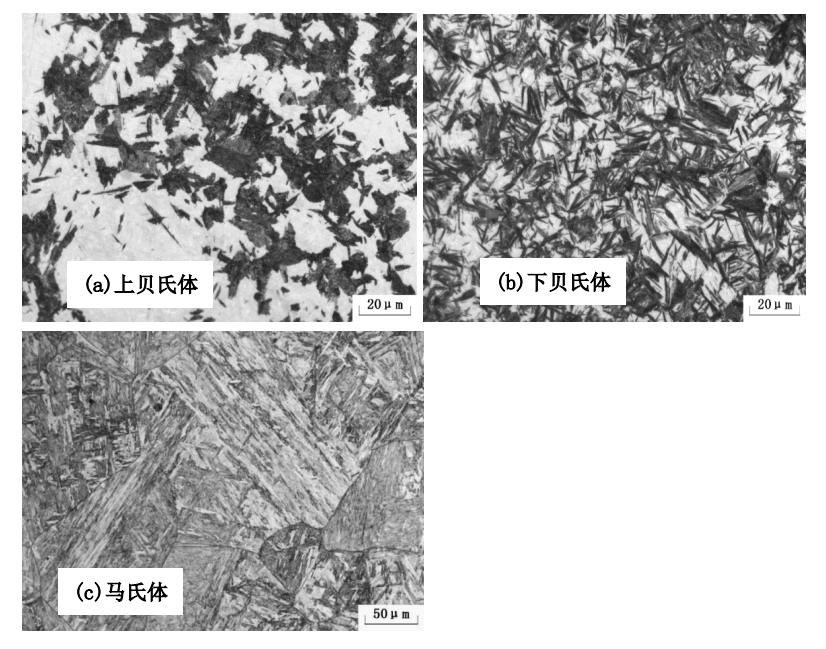
\includegraphics[width=300pt]{6.png}
\end{center}

\textbf{(二) 回火}

回火是将经过淬火的试样加热到临界点$A_1$ 以下的适当温度,保持一定时间后,采用适当的冷却方式进行冷却的热处理工艺。主要是消除内应力,获得所要求的力学性能以提高尺寸和稳定性。

① 回火马氏体:
低温回火后,颜色要比淬火马氏体深些,呈暗黑色的针状组织。 具有高的强度和硬度,同时韧性和塑性也较淬火马氏体有明显改善。

② 回火屈氏体:
中温回火后,在铁素体基体上弥散分布着微小粒状的渗碳体组织,渗碳体则呈细小的颗粒状,在光学显微镜下呈暗黑色不易分辨清楚。具有较好的强度和硬度,以及非常高的弹性性能。

③ 回火索氏体:
高温回火后,由颗粒状渗碳体和多边形的铁素体组成的组织。具有强度、韧性和塑性较好的综合机械性能。

\begin{center}
    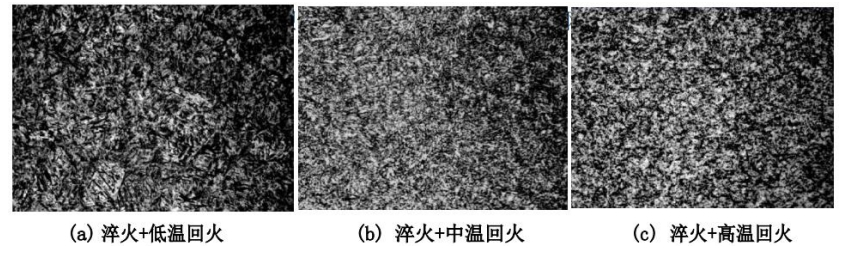
\includegraphics[width=400pt]{2.png}
\end{center}

\section*{【实验仪器】}%规格及参数
箱式电阻加热炉,洛氏硬度计,砂纸,抛光机,金相显微镜。热处理试样:
45钢及T12钢。
\section*{【实验过程】}%简述主要过程和实验内容
1、4人一组,45钢(2个)、T8(1个)及T12钢(1个),(对应下表中相应的热处理工艺方法)

\begin{center}
    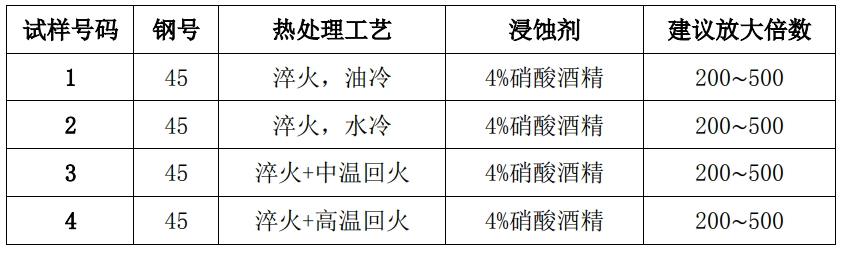
\includegraphics[width=350pt]{3.png}
\end{center}

2、制定热处理工艺参数,可参考以下工艺参数。τ = $\alpha$KD


(1. 45 钢淬火工艺:加热温度为 $860 \pm 10$℃,根据试样有效尺寸计算保温时间,保温后用长柄铁钳夹出放入\textbf{淬火油}中冷却。

(2. 45 钢淬火工艺:加热温度为 $860 \pm 10$℃,根据试样有效尺寸计算保温时间,保温后用长柄铁钳夹出放入\textbf{水}中进行冷却。

(3. 45 钢淬水+中温回火工艺:加热温度为 $860 \pm 10$℃,根据试样有效尺寸计算保温时间,保温后出炉进行水淬。随后放入炉中加热至 400℃,保温 1 个小时后出炉空冷。

(4. 45 钢淬水+高温回火工艺:加热温度为 $860 \pm 10$℃,根据试样有效尺寸计算保温时间,保温后出炉进行水淬。随后放入炉中加热至 600℃,保温 1 个小时后出炉空冷。


3、利用硬度计对所有热处理后的试样进行硬度测试,每个试样至少三个试验点,再取一个平均值,分析热处理工艺对其硬度的影响。按照下表选用硬度计。(硬度测试须在金相磨制观
察前完成)

\begin{center}
    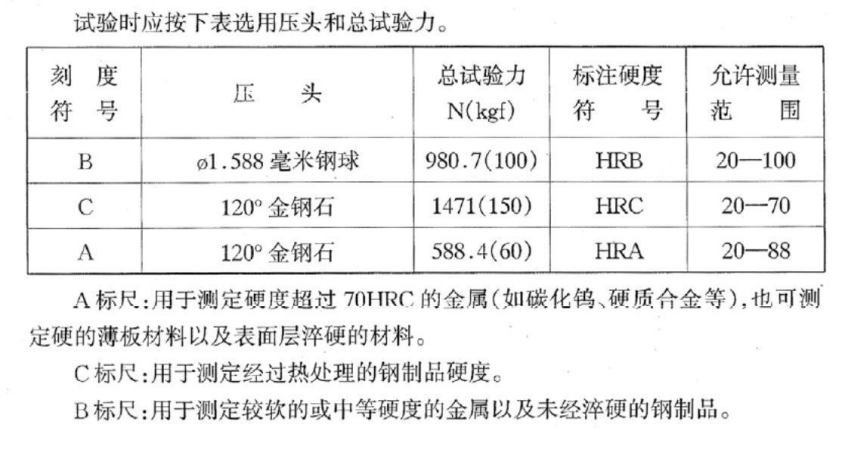
\includegraphics[width=350pt]{4.png}
\end{center}


4、根据拟定的热处理工艺对试样进行相应的热处理工艺处理,然后利用金相砂
纸对热处理后的试样进行磨制、抛光,并用4\%的硝酸酒精进行腐蚀制得金相试样。
利用金相显微镜对其进行显微组织观察,分析热处理工艺对其组织的影响。

5、实验结束后,汇总各小组实验数据,根据实验数据分析冷却方法及回火温度对碳钢性能(硬度)的影响,画出回火温度同硬度的关系曲线,并阐明硬度变化的原因。
\section*{【实验数据】}

\begin{center}
    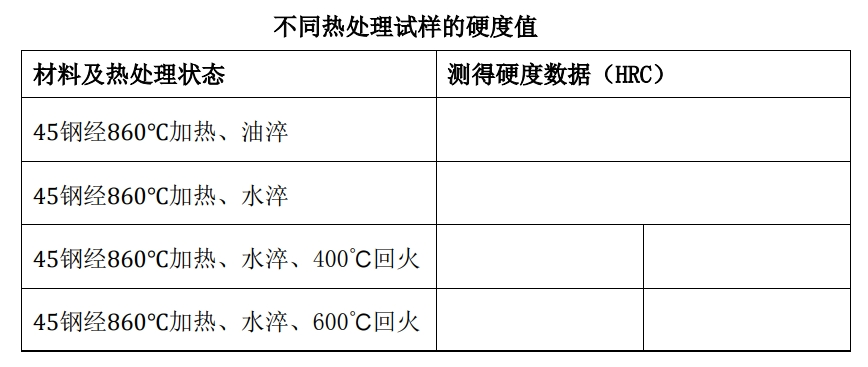
\includegraphics[width=400pt]{5.png}
\end{center}

\end{document}